%%%%%%%%%%%%%%%%%%%%%%%%%%%%%%% document and size %%%%%%%%%%%%%%%%%%%%%%%%%%%%%%
\documentclass[10pt]{beamer}

%%%%%%%%%%%%%%%%%%%%%%%%%%%%% special libraries %%%%%%%%%%%%%%%%%%%%%%%%%%%%%%%%
\usepackage{ngerman}
\usepackage{tikz}
\usetikzlibrary{arrows,automata}
\usepackage{fancyhdr}
\usepackage[export]{adjustbox}
\usepackage{lipsum}
\usepackage{lmodern}
\usepackage{tabularx}
\usepackage{array}
\usepackage{amsmath}
\usepackage[dvipsnames]{xcolor}
%%%%%%%%%%%%%%%%%%%%%%%%%%%%%% custum commands %%%%%%%%%%%%%%%%%%%%%%%%%%%%%%%%%
\newcommand{\gap}{\ \\ \ \\}
%%%%%%%%%%%%%%%%%%%%%%%%%%%%%%%%% DO NOT TOUCH %%%%%%%%%%%%%%%%%%%%%%%%%%%%%%%%%
\setbeamerfont{footnote}{size=\scriptsize}
\setbeamertemplate{footline}{}
\setbeamercolor{footnote}{fg=white,bg=mDarkTeal}


\usetheme[progressbar=frametitle]{metropolis}
\usepackage{appendixnumberbeamer}

\usepackage{booktabs}
\usepackage[scale=2]{ccicons}

\usepackage{pgfplots}
\usepgfplotslibrary{dateplot}

\usepackage{xspace}
\newcommand{\themename}{\textbf{\textsc{metropolis}}\xspace}

\title{Der Linearzeit MST Algorithmus}
\subtitle{Der schnellste Algorithmus f"ur das MST/ MSF Problem}
\date{}
\author{Max Springenberg}
\institute{Proseminar: Randomisierte Algorithmen, TU Dortmund}
%%%%%%%%%%%%%%%%%%%%%%%%%%%%%%%%%%%%%%%%%%%%%%%%%%%%%%%%%%%%%%%%%%%%%%%%%%%%%%%%

\begin{document}

%\setbeamercolor{block title}{use=structure,fg=white,bg=gray!75!black}
%\setbeamercolor{block body}{use=structure,fg=black,bg=gray!20!white}maketitle
\maketitle


%\begin{frame}{Table of contents}
%  \setbeamertemplate{section in toc}[sections numbered]
%  \tableofcontents[hideallsubsections]
%\end{frame}

% MST
% * was ist ein MST
% * was ist ein minimaler MST
\section{MST in gewichteten Graphen}
\begin{frame}{Definition MST}
    Ein Teilgraph $T$ ist genau dann ein minimaler Spannbaum von $G$, 
    wenn er ein Spannbaum in G ist und die Summe seiner Kantengewichte 
    $\underset{e \in E_T}{\sum} w(e)$ 
    minimal ist.\\
\end{frame}
\begin{frame}{Definition MST}
    Ein Teilgraph \textcolor{orange}{$T$} ist genau dann 
    ein \textcolor{orange}{minimaler Spannbaum} von $G$, 
    wenn er ein Spannbaum in G ist und die 
    Summe seiner Kantengewichte 
    \textcolor{orange}{$\underset{e \in E_T}{\sum} w(e)$ minimal} ist.\\
    \gap
    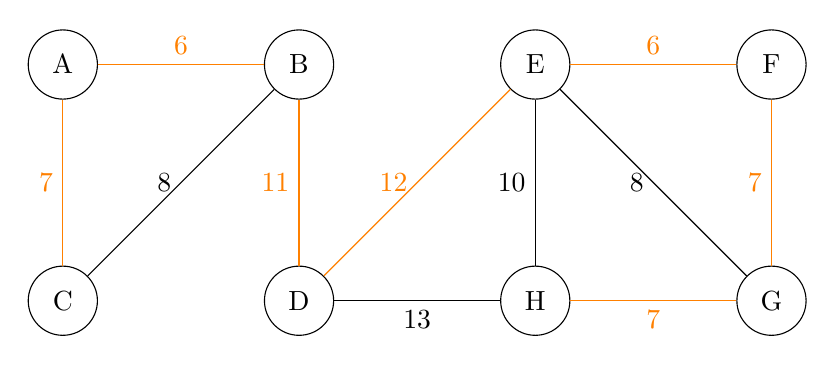
\begin{tikzpicture}
        \node[state](A) at (0,0)  {A};
        \node[state](B) at (3,0)  {B};
        \node[state](C) at (0,-3) {C};
        \node[state](D) at (3,-3) {D};
        \node[state](E) at (6,0)  {E};
        \node[state](F) at (9,0)  {F};
        \node[state](G) at (9,-3) {G};
        \node[state](H) at (6,-3) {H};
        \path
            (A) edge [-, above, color=orange] node {6}  (B)
                edge [-, left , color=orange] node {7}  (C)
            (B)                                        
                edge [-, left ] node               {8}  (C)
                edge [-, left , color=orange] node {11} (D)
            (D)                                        
                edge [-, left , color=orange] node {12} (E)
                edge [-, below] node               {13} (H)
            (E)                                        
                edge [-, above, color=orange] node {6}  (F)
                edge [-, left ] node               {8}  (G)
                edge [-, left ] node               {10} (H)
            (F)                                        
                edge [-, left , color=orange] node {7}  (G)
            (G)                                        
                edge [-, below, color=orange] node {7}  (H)
            ;
    \end{tikzpicture}
\end{frame}

% B"aume vs W"alder
% * Was ist ein Wald?
\section{B"aume vs. W"alder}
\begin{frame}{MSF}
    Ist ein Graph nicht zusammenh"angend, so kann auch ein MSF den MST ersetzen.
    Der MSF ist ein Teilgraph aus disjunkten MSTs.
    \gap
    \vtop{\vskip0pt\hbox{
        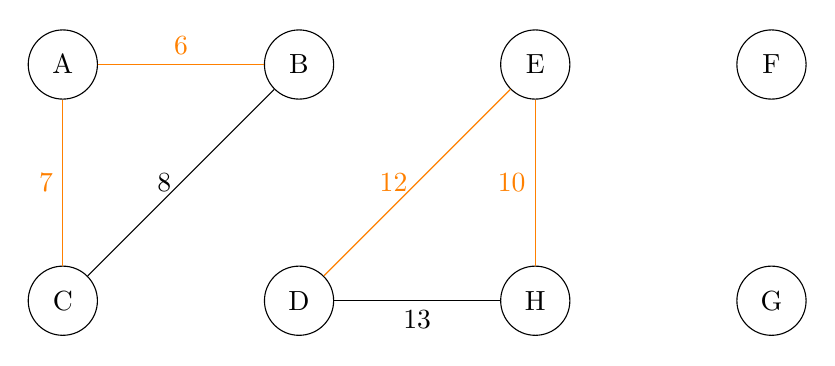
\begin{tikzpicture}
            \node[state](A) at (0,0)  {A};
            \node[state](B) at (3,0)  {B};
            \node[state](C) at (0,-3) {C};
            \node[state](D) at (3,-3) {D};
            \node[state](E) at (6,0)  {E};
            \node[state](H) at (6,-3) {H};
            \node[state](F) at (9,0)  {F};
            \node[state](G) at (9,-3) {G};
            \path
                (A) edge [-, above, color=orange] node {6} (B)
                    edge [-, left , color=orange] node {7} (C)
                (B)
                    edge [-, left] node {8} (C)
                (D)
                    edge [-, left , color=orange] node {12} (E)
                    edge [-, below] node {13} (H)
                (E)
                    edge [-, left , color=orange] node {10} (H)
                ;
        \end{tikzpicture}
    }}\\
\end{frame}

% Boruvka Phasen:
% * Wie werden zu kontraktierende Kanten ausgew"ahlt?
% * Was ist die Maximale Gr"o"se des Graphen nach einer Phase?
\section{Bor\r uvka Phasen}
\begin{frame}{Ablauf}
    \begin{enumerate}
        \item Kontraktierende Kanten markieren
        \item Verbundene Komponenten bestimmen
        \item Verbundene Komponenten durch einzelne Knoten ersetzen
        \item Selbstschleifen entfernen
    \end{enumerate}
    \gap
    \begin{block}{Was bedeutes das f"ur den reduzierten Graphen?}
    $\Rightarrow$ Knoten werden auf maximal $n/2, n = |V|$ reduziert!\\
    \end{block}
\end{frame}
\begin{frame}{1. Kontraktierende Kanten markieren}
    \begin{tikzpicture}[minND/.style={circle,
                                      anchor=center,
                                      draw=black,
                                      text width=2.5mm,
                                      inner sep=3pt,
                                      align=center,
                                      text left}]
        %\node[state](A) at (0,0)  {A};
        \node[minND](A1) at (0,0) {$A_1$};
        \node[minND](A2) at (1,0) {$A_2$};
                                         
        %\node[state](B) at (3,0)  {B};  
        \node[minND](B1) at (3,0) {$B_1$};
        \node[minND](B2) at (4,0) {$B_2$};

        %\node[state](C) at (0,-3) {C};
        \node[minND](C1) at (0,-3) {$C_1$};
        \node[minND](C2) at (0,-4) {$C_2$};
;
        %\node[state](D) at (3,-3) {D};
        \node[minND](D1) at (3,-3) {$D_1$};
        \node[minND](D2) at (3,-4) {$D_2$};
;
        %\node[state](E) at (6,0)  {E};
        \node[minND](E1) at (6,0) {$E_1$};
        \node[minND](E2) at (7,0) {$E_2$};
;
        %\node[state](F) at (9,0)  {F};
        \node[minND](F1) at (9,0)  {$F_1$};
        \node[minND](F2) at (10,0) {$F_2$};
;
        %\node[state](G) at (9,-3) {G};
        \node[minND](G1) at (9,-3) {$G_1$};
        \node[minND](G2) at (9,-4) {$G_2$};
;
        %\node[state](H) at (6,-3) {H};
        \node[minND](H1) at (6,-3) {$H_1$};
        \node[minND](H2) at (6,-4) {$H_2$};

        \path
            %(A) edge [-, above] node {6} (B)
            %    edge [-, left ] node {7} (C)
            (A1)
                edge [-, above, color=blue] node {3} (A2)
                edge [-, left ] node {7} (C1)
            (A2)
                edge [-, above] node {6} (B1)
            %(B)
            %    edge [-, left ] node {8} (C)
            %    edge [-, left ] node {11} (D)
            (B1)
                edge [-, above, color=blue] node {5} (B2)
                edge [-, left ] node {8}  (C1)
                edge [-, left ] node {11} (D1)
            % (C) //
            (C1)
                edge [-, left , color=blue] node {6} (C2)
            %(D)
            %    edge [-, left ] node {12} (E)
            %    edge [-, below] node {13} (H)
            (D1)
                edge [-, left , color=blue] node {10} (D2)
                edge [-, left ] node {12} (E1)
            (D2)
                edge [-, below] node {13} (H2)
            %(E)
            %    edge [-, above] node {6} (F)
            %    edge [-, left ] node {8} (G)
            %    edge [-, left ] node {10} (H)
            (E1)
                edge [-, above, color=blue] node {1} (E2)
                edge [-, left ] node {8} (G1)
                edge [-, left ] node {10} (H1)
            (E2)
                edge [-, above] node {6} (F1)
            %(F)
            %    edge [-, left ] node {7} (G)
            (F1)
                edge [-, above, color=blue] node {3} (F2)
            (F2)
                edge [-, left ] node {7} (G1)
            %(G)
            %    edge [-, below] node {7} (H)
            (G1)
                edge [-, left , color=blue] node {5} (G2)
            (G2)
                edge [-, below] node {7} (H2)
            % (H) \\
            (H1)
                edge [-, left , color=blue] node {4} (H2)
            ;
    \end{tikzpicture}
\end{frame}
\begin{frame}{2. Verbundene Komponenten bestimmen}
    \begin{tikzpicture}[minND/.style={circle,
                                      anchor=center,
                                      draw=black,
                                      text width=2.5mm,
                                      inner sep=3pt,
                                      align=center,
                                      text left}]
        %\node[state](A) at (0,0)  {A};
        \node[minND](A1) at (0,0) {$A_1$};
        \node[minND](A2) at (1,0) {$A_2$};
                                         
        %\node[state](B) at (3,0)  {B};  
        \node[minND, color=brown](B1) at (3,0) {$B_1$};
        \node[minND, color=brown](B2) at (4,0) {$B_2$};

        %\node[state](C) at (0,-3) {C};
        \node[minND, red](C1) at (0,-3) {$C_1$};
        \node[minND, red](C2) at (0,-4) {$C_2$};
;
        %\node[state](D) at (3,-3) {D};
        \node[minND, orange](D1) at (3,-3) {$D_1$};
        \node[minND, orange](D2) at (3,-4) {$D_2$};
;
        %\node[state](E) at (6,0)  {E};
        \node[minND, green](E1) at (6,0) {$E_1$};
        \node[minND, green](E2) at (7,0) {$E_2$};
;
        %\node[state](F) at (9,0)  {F};
        \node[minND, purple](F1) at (9,0)  {$F_1$};
        \node[minND, purple](F2) at (10,0) {$F_2$};
;
        %\node[state](G) at (9,-3) {G};
        \node[minND, gray](G1) at (9,-3) {$G_1$};
        \node[minND, gray](G2) at (9,-4) {$G_2$};
;
        %\node[state](H) at (6,-3) {H};
        \node[minND, violet](H1) at (6,-3) {$H_1$};
        \node[minND, violet](H2) at (6,-4) {$H_2$};

        \path
            %(A) edge [-, above] node {6} (B)
            %    edge [-, left ] node {7} (C)
            (A1)
                edge [-, above, color=blue] node {3} (A2)
                edge [-, left ] node {7} (C1)
            (A2)
                edge [-, above] node {6} (B1)
            %(B)
            %    edge [-, left ] node {8} (C)
            %    edge [-, left ] node {11} (D)
            (B1)
                edge [-, above, color=blue] node {5} (B2)
                edge [-, left ] node {8}  (C1)
                edge [-, left ] node {11} (D1)
            % (C) //
            (C1)
                edge [-, left , color=blue] node {6} (C2)
            %(D)
            %    edge [-, left ] node {12} (E)
            %    edge [-, below] node {13} (H)
            (D1)
                edge [-, left , color=blue] node {10} (D2)
                edge [-, left ] node {12} (E1)
            (D2)
                edge [-, below] node {13} (H2)
            %(E)
            %    edge [-, above] node {6} (F)
            %    edge [-, left ] node {8} (G)
            %    edge [-, left ] node {10} (H)
            (E1)
                edge [-, above, color=blue] node {1} (E2)
                edge [-, left ] node {8} (G1)
                edge [-, left ] node {10} (H1)
            (E2)
                edge [-, above] node {6} (F1)
            %(F)
            %    edge [-, left ] node {7} (G)
            (F1)
                edge [-, above, color=blue] node {3} (F2)
            (F2)
                edge [-, left ] node {7} (G1)
            %(G)
            %    edge [-, below] node {7} (H)
            (G1)
                edge [-, left , color=blue] node {5} (G2)
            (G2)
                edge [-, below] node {7} (H2)
            % (H) \\
            (H1)
                edge [-, left , color=blue] node {4} (H2)
            ;
    \end{tikzpicture}
\end{frame}
\begin{frame}{3. Verbundene Komponenten durch einzelne Knoten ersetzen}
    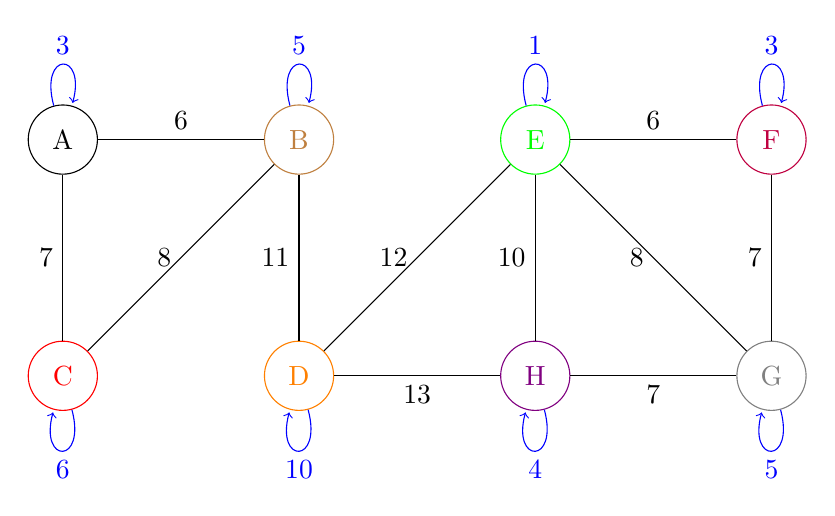
\begin{tikzpicture}
        \node[state](A) at (0,0)  {A};
        \node[state, brown](B) at (3,0)  {B};
        \node[state, red](C) at (0,-3) {C};
        \node[state, orange](D) at (3,-3) {D};
        \node[state, green](E) at (6,0)  {E};
        \node[state, purple](F) at (9,0)  {F};
        \node[state, gray](G) at (9,-3) {G};
        \node[state, violet](H) at (6,-3) {H};
        \path
            (A) edge [-, above] node {6} (B)
                edge [-, left ] node {7} (C)
                edge [-, loop above, color=blue] node {3} (A)
            (B)
                edge [-, left ] node {8} (C)
                edge [-, left ] node {11} (D)
                edge [-, loop above, color=blue] node {5} (B)
            (C)
                edge [-, loop below, color=blue] node {6} (C)
            (D)
                edge [-, left ] node {12} (E)
                edge [-, below] node {13} (H)
                edge [-, loop below, color=blue] node {10} (D)
            (E)
                edge [-, above] node {6} (F)
                edge [-, left ] node {8} (G)
                edge [-, left ] node {10} (H)
                edge [-, loop above, color=blue] node {1} (E)
            (F)
                edge [-, left ] node {7} (G)
                edge [-, loop above, color=blue] node {3} (F)
            (G)
                edge [-, below] node {7} (H)
                edge [-, loop below, color=blue] node {5} (G)
            (H)
                edge [-, loop below, color=blue] node {4} (H)
            ;
    \end{tikzpicture}
\end{frame}
\begin{frame}{4. Selbstschleifen entfernen}
    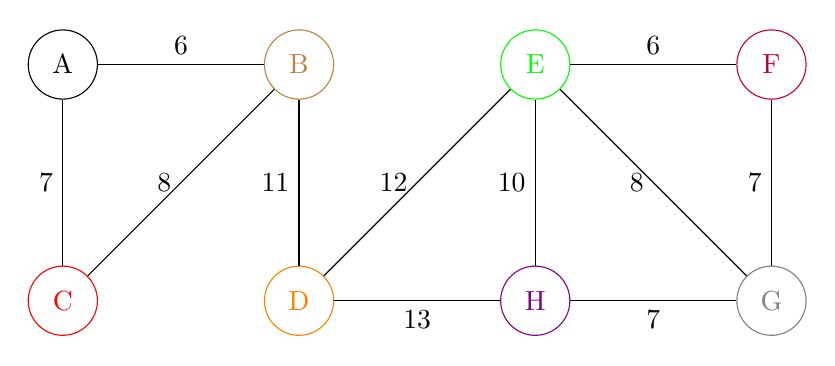
\begin{tikzpicture}
        \node[state](A) at (0,0)  {A};
        \node[state, brown](B) at (3,0)  {B};
        \node[state, red](C) at (0,-3) {C};
        \node[state, orange](D) at (3,-3) {D};
        \node[state, green](E) at (6,0)  {E};
        \node[state, purple](F) at (9,0)  {F};
        \node[state, gray](G) at (9,-3) {G};
        \node[state, violet](H) at (6,-3) {H};
        \path
            (A) edge [-, above] node {6} (B)
                edge [-, left ] node {7} (C)
            (B)
                edge [-, left ] node {8} (C)
                edge [-, left ] node {11} (D)
            (D)
                edge [-, left ] node {12} (E)
                edge [-, below] node {13} (H)
            (E)
                edge [-, above] node {6} (F)
                edge [-, left ] node {8} (G)
                edge [-, left ] node {10} (H)
            (F)
                edge [-, left ] node {7} (G)
            (G)
                edge [-, below] node {7} (H)
            ;
    \end{tikzpicture}
\end{frame}





% F-schwere/ leichte Kanten
% * wann ist eine Kante F-schwer
% * wann ist sie F-leicht
% * kann eine F-schwere Kante im MST enthalten sein?
\section{F-schwere/ -leichte Kanten}
\begin{frame}{Definition}
    Sei $P(e=\{u,v\})$ der Pfad, der die Knoten $u,v$ im MSF verbindet (in Kanten)\\
    Sei $w : E \rightarrow \mathbb{R}$, die Gewichtsfunktion von G\\
    Sei ferner definiert $w(E) = \{w(e_1), \ldots, w(e_m)\}$
    \gap
    Eine Kante ist F-schwer, wenn gilt:
    $$
        \textcolor{orange}{w(e) > w_F(e)}
    $$
    , wobei:\\
    $w_F(e=(u,v))$ = \begin{cases}
                        $\infty$, $u$ und $v$ sind in verschiedenen Komponenten\\
                                $\textcolor{orange}{max\{w(P(e))\}}$, sonst 
                     \end{cases}
\end{frame}

% Randomisierte Stichproben
% * `w"urfeln` erkl"aren
\section{Randomiserte Stichprobem}

% Wie k"onnen 
\begin{frame}
    \begin{tabular}{lp{6cm}}
        \fontsize{18}{10} \selectfont Wirf eine M"unze!
        &\vcenter{\vskip0pt
                  \hbox{
\includegraphics[height=60mm, left]{coin-flip-clipart.pdf}}}\\
        &\fontsize{5}{10} \selectfont
            Quelle: https://melbournechapter.net/explore/coin-flip-clipart/\\
    \end{tabular}
\end{frame}

\begin{frame}{Kanten `w"urfeln`}
    \hfill \begin{tabular}{rr}
        \textcolor{gray}{$G$}:&\vtop{\vskip0pt\hbox{
        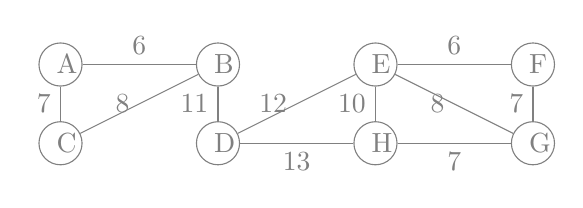
\begin{tikzpicture}[minND/.style={circle,
                                          draw=gray,
                                          text width=1mm,
                                          inner sep=3pt,
                                          align=center,
                                          text centered},
                            color=gray]
            \node[minND](A) at (0,0)  {A};
            \node[minND](B) at (2,0)  {B};
            \node[minND](C) at (0,-1) {C};
            \node[minND](D) at (2,-1) {D};
            \node[minND](E) at (4,0)  {E};
            \node[minND](F) at (6,0)  {F};
            \node[minND](G) at (6,-1) {G};
            \node[minND](H) at (4,-1) {H};
            \path
                (A) edge [-, above] node {6}  (B)
                    edge [-, left ] node {7}  (C)
                (B)                          
                    edge [-, left ] node {8}  (C)
                    edge [-, left ] node {11} (D)
                (D)                          
                    edge [-, left ] node {12} (E)
                    edge [-, below] node {13} (H)
                (E)                          
                    edge [-, above] node {6}  (F)
                    edge [-, left ] node {8}  (G)
                    edge [-, left ] node {10} (H)
                (F)                          
                    edge [-, left ] node {7}  (G)
                (G)                          
                    edge [-, below] node {7}  (H)
                ;
        \end{tikzpicture}
        }}\\
    \end{tabular}\\
    \gap
    \begin{tabular}{ll}
        $G(p=0,5):$\\
        \vtop{\vskip0pt\hbox{
        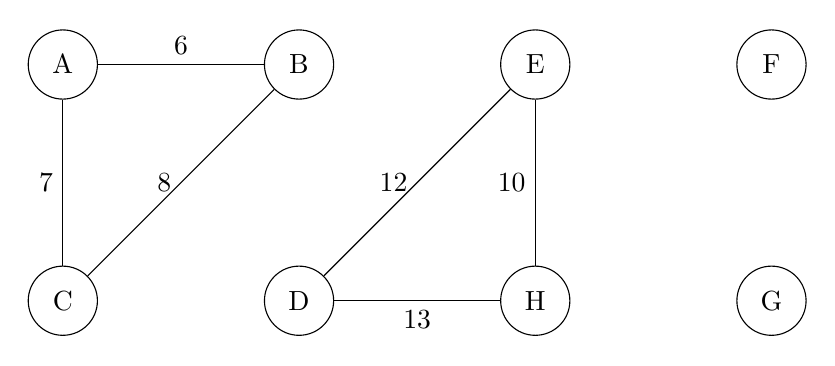
\begin{tikzpicture}
            \node[state](A) at (0,0)  {A};
            \node[state](B) at (3,0)  {B};
            \node[state](C) at (0,-3) {C};
            \node[state](D) at (3,-3) {D};
            \node[state](E) at (6,0)  {E};
            \node[state](H) at (6,-3) {H};
            \node[state](F) at (9,0)  {F};
            \node[state](G) at (9,-3) {G};
            \path
                (A) edge [-, above] node {6} (B)
                    edge [-, left ] node {7} (C)
                (B)
                    edge [-, left ] node {8} (C)
                (D)
                    edge [-, left ] node {12} (E)
                    edge [-, below] node {13} (H)
                (E)
                    edge [-, left ] node {10} (H)
                ;
        \end{tikzpicture}
    }}\\
    \end{tabular}
\end{frame}
\begin{frame}{MST vs. MSF}
    \hfill \begin{tabular}{rr}
            \textcolor{gray}{$MST_{G}$:}&\vtop{\vskip0pt\hbox{
            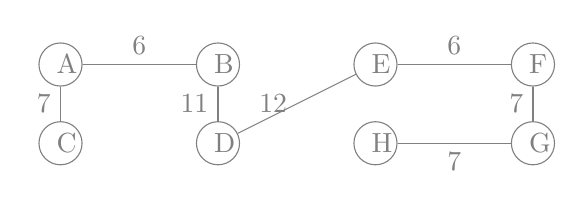
\begin{tikzpicture}[minND/.style={circle,
                                          draw=gray,
                                          text width=1mm,
                                          inner sep=3pt,
                                          align=center,
                                          text centered},
                            color=gray]
                \node[minND](A) at (0,0)  {A};
                \node[minND](B) at (2,0)  {B};
                \node[minND](C) at (0,-1) {C};
                \node[minND](D) at (2,-1) {D};
                \node[minND](E) at (4,0)  {E};
                \node[minND](F) at (6,0)  {F};
                \node[minND](G) at (6,-1) {G};
                \node[minND](H) at (4,-1) {H};
                \path
                    (A) edge [-, above] node {6}  (B)
                        edge [-, left ] node {7}  (C)
                    (B)                          
                        edge [-, left ] node {11} (D)
                    (D)                          
                        edge [-, left ] node {12} (E)
                    (E)                          
                        edge [-, above] node {6}  (F)
                    (F)                          
                        edge [-, left ] node {7}  (G)
                    (G)                          
                        edge [-, below] node {7}  (H)
                    ;
            \end{tikzpicture}
    }}\\
    \end{tabular}\\
    \begin{tabular}{ll}
        $MSF_{G(0,5)}:$\\
        \vtop{\vskip0pt\hbox{
        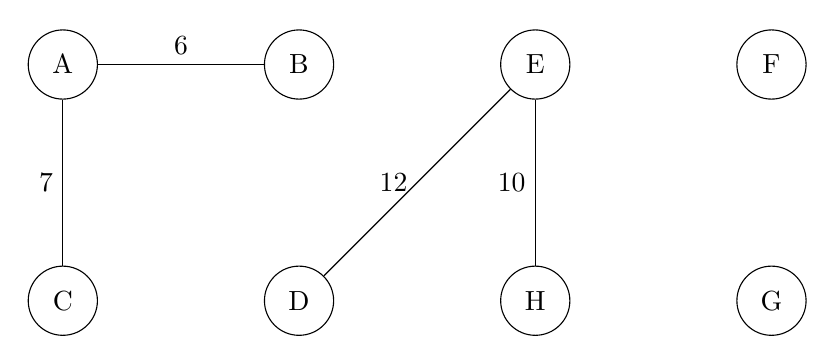
\begin{tikzpicture}
            \node[state](A) at (0,0)  {A};
            \node[state](B) at (3,0)  {B};
            \node[state](C) at (0,-3) {C};
            \node[state](D) at (3,-3) {D};
            \node[state](E) at (6,0)  {E};
            \node[state](H) at (6,-3) {H};
            \node[state](F) at (9,0)  {F};
            \node[state](G) at (9,-3) {G};
            \path
                (A) edge [-, above] node {6} (B)
                    edge [-, left ] node {7} (C)
                (D)
                    edge [-, left ] node {12} (E)
                (E)
                    edge [-, left ] node {10} (H)
                ;
        \end{tikzpicture}
    }}\\
    \end{tabular}
\end{frame}

\section{Erkenntnis}
\begin{frame}{Eleminierung von unn"utzen Kanten}
    \hfill \begin{tabular}{ll}
        \textcolor{gray}{$MSF_{G(0,5)}$:}&\vtop{\vskip0pt\hbox{
        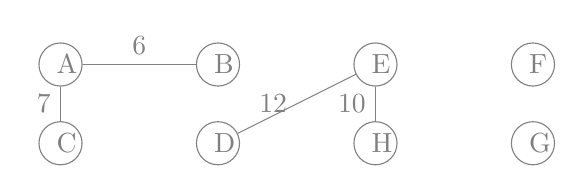
\begin{tikzpicture}[minND/.style={circle,
                                          draw=gray,
                                          text width=1mm,
                                          inner sep=3pt,
                                          align=center,
                                          text centered},
                            color=gray]
            \node[minND](A) at (0,0)  {A};
            \node[minND](B) at (2,0)  {B};
            \node[minND](C) at (0,-1) {C};
            \node[minND](D) at (2,-1) {D};
            \node[minND](E) at (4,0)  {E};
            \node[minND](H) at (4,-1) {H};
            \node[minND](F) at (6,0)  {F};
            \node[minND](G) at (6,-1) {G};
            \path
                (A) edge [-, above] node {6} (B)
                    edge [-, left ] node {7} (C)
                (D)
                    edge [-, left ] node {12} (E)
                (E)
                    edge [-, left ] node {10} (H)
                ;
        \end{tikzpicture}
    }}\\
    \end{tabular}\\
    \gap
    \begin{tabular}{ll}
        $G:$&\vtop{\vskip0pt\hbox{
        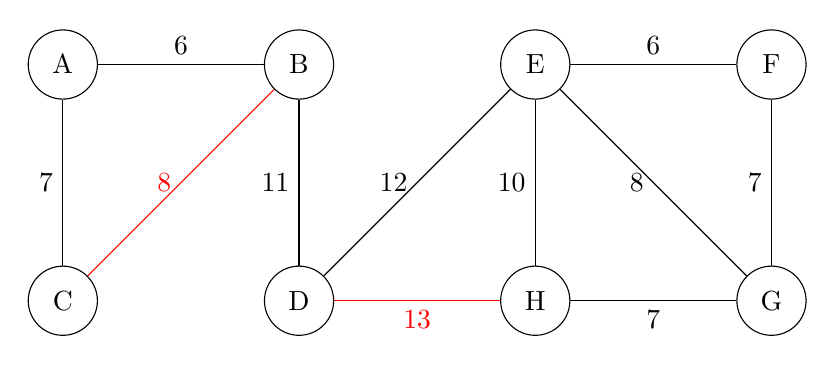
\begin{tikzpicture}
            \node[state](A) at (0,0)  {A};
            \node[state](B) at (3,0)  {B};
            \node[state](C) at (0,-3) {C};
            \node[state](D) at (3,-3) {D};
            \node[state](E) at (6,0)  {E};
            \node[state](F) at (9,0)  {F};
            \node[state](G) at (9,-3) {G};
            \node[state](H) at (6,-3) {H};
            \path
                (A) edge [-, above] node            {6}  (B)
                    edge [-, left ] node            {7}  (C)
                (B)                                     
                    edge [-, left , color=red] node {8}  (C)
                    edge [-, left ] node            {11} (D)
                (D)                                     
                    edge [-, left ] node            {12} (E)
                    edge [-, below, color=red] node {13} (H)
                (E)                                     
                    edge [-, above] node            {6}  (F)
                    edge [-, left ] node            {8}  (G)
                    edge [-, left ] node            {10} (H)
                (F)                                     
                    edge [-, left ] node            {7}  (G)
                (G)                                     
                    edge [-, below] node            {7}  (H)
                ;
        \end{tikzpicture}
        }}\\
    \end{tabular}
\end{frame}
%\begin{frame}
%    \hfill \begin{tabular}{llll}
%        \textcolor{gray}{$G(p=0,5):$}&\vtop{\vskip0pt\hbox{
%        \begin{tikzpicture}[minND/.style={circle,
%                                          draw=gray,
%                                          text width=1mm,
%                                          inner sep=3pt,
%                                          align=center,
%                                          text centered},
%                            color=gray]
%            \node[minND](A) at (0,0)  {A};
%            \node[minND](B) at (1,0)  {B};
%            \node[minND](C) at (0,-1) {C};
%            \node[minND](D) at (1,-1) {D};
%            \node[minND](E) at (2,0)  {E};
%            \node[minND](H) at (2,-1) {H};
%            \path
%                (A) edge [-, above] node {1} (B)
%                    edge [-, left ] node {2} (C)
%                (B)
%                    edge [-, left ] node {3} (C)
%                (D)
%                    edge [-, left ] node {7} (E)
%                    edge [-, below] node {8} (H)
%                (E)
%                    edge [-, left ] node {5} (H)
%                ;
%        \end{tikzpicture}
%    }}
%        &\textcolor{gray}{$G:$}&\vtop{\vskip0pt\hbox{
%        \begin{tikzpicture}[minND/.style={circle,
%                                          draw=gray,
%                                          text width=1mm,
%                                          inner sep=3pt,
%                                          align=center,
%                                          text centered},
%                            color=gray]
%            \node[minND](A) at (0,0)  {A};
%            \node[minND](B) at (1,0)  {B};
%            \node[minND](C) at (0,-1) {C};
%            \node[minND](D) at (1,-1) {D};
%            \node[minND](E) at (2,0)  {E};
%            \node[minND](F) at (3,0)  {F};
%            \node[minND](G) at (3,-1) {G};
%            \node[minND](H) at (2,-1) {H};
%            \path
%                (A) edge [-, above] node {1} (B)
%                    edge [-, left ] node {2} (C)
%                (B)
%                    edge [-, left , color=red] node {3} (C)
%                    edge [-, left ] node {6} (D)
%                (D)
%                    edge [-, left ] node {7} (E)
%                    edge [-, below, color=red] node {8} (H)
%                (E)
%                    edge [-, above] node {1} (F)
%                    edge [-, left ] node {3} (G)
%                    edge [-, left ] node {5} (H)
%                (F)
%                    edge [-, left ] node {2} (G)
%                (G)
%                    edge [-, below] node {2} (H)
%                ;
%        \end{tikzpicture}
%        }}\\
%    $\ldots$ doch:\\
%    \end{tabular}
%    \begin{itemize}
%        \item Wie erreicht man dadurch lineare Laufzeit?
%        \item Wie kann ein vern"unftiger Spannbaum nach eliminierung von Kanten
%              garantiert sein?
%    \end{itemize}\\
%\end{frame}
\begin{frame}{Idee}
    \begin{enumerate}
        \item Nutze Bor\r uvka-Phasen, um die Anzahl von Knoten zu reduzieren
        \item Nutze Stichproben, um die Anzahl von Kanten zu reduzieren
        \item Entferne alle F-schweren Kanten
        \item \textbf{Rekursion}
    \end{enumerate}\\
\end{frame}
\begin{frame}{Teaser}
    \begin{itemize}
        \item Wie fassen wir die Erkenntnis geschickt in einem Algorithmus?
        \item Wie erhalten wir trotz rekursiven Aufrufen eine erwartete lineare
              Laufzeit?
    \end{itemize}
\end{frame}
\end{document}
